\documentclass[ngerman,bibliography=totoc,oneside,12pt,a4paper]{scrbook}
\usepackage{lmodern}
\usepackage{amssymb,amsmath}
\usepackage{ifxetex,ifluatex}
\usepackage{fixltx2e} % provides \textsubscript
\ifnum 0\ifxetex 1\fi\ifluatex 1\fi=0 % if pdftex
  \usepackage[T1]{fontenc}
  \usepackage[utf8]{inputenc}
\else % if luatex or xelatex
  \ifxetex
    \usepackage{mathspec}
  \else
    \usepackage{fontspec}
  \fi
  \defaultfontfeatures{Ligatures=TeX,Scale=MatchLowercase}
\fi
% use upquote if available, for straight quotes in verbatim environments
\IfFileExists{upquote.sty}{\usepackage{upquote}}{}
% use microtype if available
\IfFileExists{microtype.sty}{%
\usepackage[]{microtype}
\UseMicrotypeSet[protrusion]{basicmath} % disable protrusion for tt fonts
}{}
\PassOptionsToPackage{hyphens}{url} % url is loaded by hyperref
\usepackage[unicode=true]{hyperref}
\hypersetup{
            pdftitle={Kompendium zum wissenschaftlichen Arbeiten},
            pdfauthor={Thomas Janßen},
            pdfborder={0 0 0},
            breaklinks=true}
\urlstyle{same}  % don't use monospace font for urls
\ifnum 0\ifxetex 1\fi\ifluatex 1\fi=0 % if pdftex
  \usepackage[shorthands=off,main=ngerman]{babel}
\else
  \usepackage{polyglossia}
  \setmainlanguage[]{german}
\fi
\usepackage[style=apa,refsegment=chapter]{biblatex}
\addbibresource{literatur.bib}
\usepackage{longtable,booktabs}
% Fix footnotes in tables (requires footnote package)
\IfFileExists{footnote.sty}{\usepackage{footnote}\makesavenoteenv{long table}}{}
\usepackage{graphicx,grffile}
\makeatletter
\def\maxwidth{\ifdim\Gin@nat@width>\linewidth\linewidth\else\Gin@nat@width\fi}
\def\maxheight{\ifdim\Gin@nat@height>\textheight\textheight\else\Gin@nat@height\fi}
\makeatother
% Scale images if necessary, so that they will not overflow the page
% margins by default, and it is still possible to overwrite the defaults
% using explicit options in \includegraphics[width, height, ...]{}
\setkeys{Gin}{width=\maxwidth,height=\maxheight,keepaspectratio}
\IfFileExists{parskip.sty}{%
\usepackage{parskip}
}{% else
\setlength{\parindent}{0pt}
\setlength{\parskip}{6pt plus 2pt minus 1pt}
}
\setlength{\emergencystretch}{3em}  % prevent overfull lines
\providecommand{\tightlist}{%
  \setlength{\itemsep}{0pt}\setlength{\parskip}{0pt}}
\setcounter{secnumdepth}{5}
% Redefines (sub)paragraphs to behave more like sections
\ifx\paragraph\undefined\else
\let\oldparagraph\paragraph
\renewcommand{\paragraph}[1]{\oldparagraph{#1}\mbox{}}
\fi
\ifx\subparagraph\undefined\else
\let\oldsubparagraph\subparagraph
\renewcommand{\subparagraph}[1]{\oldsubparagraph{#1}\mbox{}}
\fi

% set default figure placement to htbp
\makeatletter
\def\fps@figure{htbp}
\makeatother

\defbibheading{bibintoc}[\bibname]{%
  \addchap{#1}}
\PassOptionsToPackage{toc=bib}{biblatex}
\usepackage{booktabs}
\usepackage{amsthm}
\usepackage[tt=false]{libertine}
\setmonofont{consolas}
\usepackage{microtype}
\usepackage{csquotes}             %für richtige Anführungszeichen
\usepackage{hanging}								%ermöglicht hängenden Einzug

%KOPFZEILE
\usepackage[automark] {scrpage2}            % Kopf- und Fußzeilen
\pagestyle{scrheadings}                % [] - erste Seite, {} - alle anderen
\setkomafont{pageheadfoot}{}
%\ihead[]{\Titel~}                      % linke Kopfzeile
\chead[]{}                              % mittlere Kopfzeile, leer
\ohead[]{}                    % rechte Kopfzeile
%\ifoot[]{}                              % linke Fußzeile
\cfoot[]{}                              % mittlere Fußzeile
\ofoot[\pagemark]{\pagemark}                              % rechte Fußzeile
%\setheadtopline{.4pt}                  % Linien über/ unter Kopf-/ Fußzeile
%\setheadsepline{1.2pt}
%\setfootsepline{2pt}
%\setfootbotline{.4pt}
\setlength\parindent{0pt}
\makeatletter
\def\thm@space@setup{%
  \thm@preskip=8pt plus 2pt minus 4pt
  \thm@postskip=\thm@preskip
}
\makeatother

\title{Kompendium zum wissenschaftlichen Arbeiten}
\providecommand{\subtitle}[1]{}
\subtitle{herausgegeben von der AG Didaktik im Fachbereich 3 der Universität
Bremen}
\author{Thomas Janßen}
\date{Version 7 · Oktober 2018}

\begin{document}
\maketitle

{
\setcounter{tocdepth}{1}
\tableofcontents
}
\chapter*{Vorwort}\label{vorwort}
\addcontentsline{toc}{chapter}{Vorwort}

Liebe Student\_innen,

in Anlehnung an den Studiengang Politikwissenschaft, der seinen
Studierenden schon lange ein Kompendium zum Wissenschaftlichen Arbeiten
an die Hand gibt \autocite{autorengruppe2012}, bieten auch wir in der AG
Didaktik unseren Studierenden seit 2013 ein solches Machwerk an.

Primäre Motivation ist es, Ihnen eine verlässliche Information darüber
zu geben, welche wissenschaftlichen Standards wir in der AG Didaktik für
selbstverständlich halten und dementsprechend in Haus-, Bachelor- und
Masterarbeiten anlegen. Nach einer Vorstellung der Arbeitsgruppe besteht
der Kern dieses Kompendiums daher in einer Kurzanleitung zum richtigen
Zitieren. Zusätzlich haben wir einige Informationen zusammengestellt,
die Ihnen helfen können, nicht nur formal korrekte, sondern auch
wirklich gute Arbeiten zu schreiben: Sie finden einen Leitfaden zum
Schreiben von Hausarbeiten, einen kurzen Überblick darüber, was Sie
beachten müssen, wenn Sie mit personenbezogenen Daten (etwa von
Schüler\_innen) arbeiten, sowie eine Auflistung von Online-Ressourcen,
die Ihnen den Zugang zur Mathematikdidaktik erleichtern können.

Das Kompendium kann und soll im praktischen Gebrauch reifen, und so
freuen wir uns über Hinweise darauf, welche Informationen unter
Umständen noch fehlen. Sprechen Sie mich gerne persönlich an oder
schreiben Sie mir eine E-Mail an
\href{mailto:janssent@uni-bremen.de}{\nolinkurl{janssent@uni-bremen.de}}.

Ansonsten arbeiten wir von uns aus daran, das Kompendium reichhaltiger
und zugänglicher zu machen. Da die meisten von Ihnen wahrscheinlich
ohnehin am Computer arbeiten, erschien uns ein PDF nicht mehr das
optimale Format. Stattdessen ist das Kompendium ab sofort als
Online-Buch auf unserer Homepage abzurufen.\footnote{Bei der Umsetzung
  war uns Moritz Bergenthal behilflich, dessen Stelle das
  \href{https://www.uni-bremen.de/zmml/}{Zentrum für Multimedia in der
  Lehre} im Rahmen des
  \href{https://www.uni-bremen.de/zmml/projekte/win-a-tutor-e-learning-anwendungsszenarien/}{Win
  a tutor-Programms} gefördert hat.} Wer es jedoch ausdrucken oder auf
einem E-Book-Reader lesen möchte, kann mit einem Klick auf das
entsprechende Symbol in der Leiste oben ein PDF oder eine epub-Datei
herunterladen. Im Zuge dieser Modernisierung schreiben wir die meisten
Weblinks nicht mehr aus -- wenn Sie sich also beim Lesen Ihres Ausdrucks
fragen, wie Sie nun eine bestimmte Webseite erreichen, finden Sie im
Online-Dokument oder in der PDF-Datei einen klickbaren Link.

Viel Freude und Erfolg im Studium wünscht Ihnen im Namen aller
Mitglieder der AG Didaktik

Thomas Janßen

\begin{center}\rule{0.5\linewidth}{\linethickness}\end{center}

\begin{quote}
Dieses Kompendium unterliegt der Lizenz \emph{Creative Commons Zero v1.0
Universal}, die unter
\url{https://github.com/janssent/kompendium-bkdwn/blob/master/LICENSE}
eingesehen werden kann. Es darf damit in sämtlichen Formaten frei
verwendet und weiterentwickelt werden. Insbesondere besteht die
Möglichkeit, ausgehend vom unter
\url{https://github.com/janssent/kompendium-bkdwn} bereitgestellten
Quellcode eine eigene Version zu entwickeln.
\end{quote}

\chapter{Die Mathematikdidaktik an der Universität
Bremen}\label{die-mathematikdidaktik-an-der-universitat-bremen}

\section{Die AG Didaktik}\label{die-ag-didaktik}

Die AG Didaktik im Fachbereich 3 umfasst alle diejenigen
Mitarbeiter\_innen, die sich in Forschung und Lehre mit der Didaktik der
Mathematik auseinandersetzen. Geleitet wird diese Gruppe von
Prof.~Dr.~Christine Knipping und Prof.~Dr.~Maike Vollstedt. Langjährige
Erfahrungen in der Schulpraxis, in der Förderung von Lernenden und in
der Aus- und Fortbildung von Lehrkräften, vielfältige Erfahrungen in der
mathematischen und mathematikdidaktischen Forschung kommen in unserer AG
Didaktik der Mathematik zusammen. Die Vielfalt unserer Kompetenzen
nutzen wir, um im Rahmen von Lehrer\_innenausbildung und
mathematikdidaktischer Forschung mit- und voneinander zu lernen. Unser
gemeinsames Forschungsinteresse ist es, mehr theoretische und praktische
Einsicht in Prozesse der mathematischen Wissenskonstruktion und deren
fördernde und behindernde Bedingungen zu gewinnen.

\begin{figure}
\centering
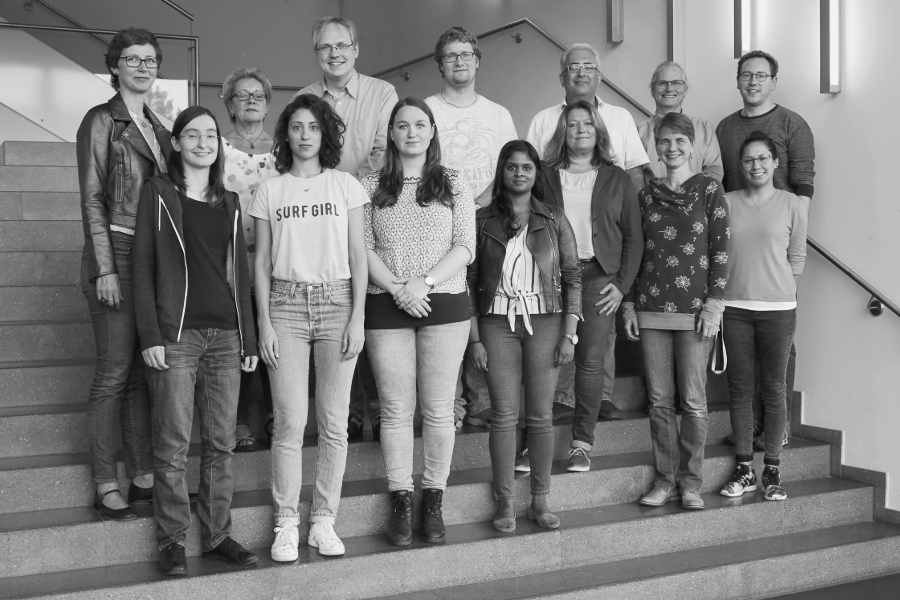
\includegraphics{ag_web_bw.jpg}
\caption{\label{fig:ID}Die Mitglieder der AG Didaktik. Es fehlen Angelika
Bikner-Ahsbahs, Uwe Schallmeier, Daniela Schansker und Mareike Best.}
\end{figure}

Zentraler Grundsatz in der Lehrer\_innenausbildung ist eine möglichst
enge Verzahnung von theoretischem und praktischem Wissen. Das bedeutet:

\begin{itemize}
\item
  eine möglichst frühe Einbindung von Studierenden in die
  mathematikdidaktische Forschung,
\item
  das Aufgreifen von Forschungsergebnissen in die praxisbezogene
  Ausbildung,
\item
  das Aufnehmen von Praxiserfahrungen in die elementarmathematische und
  mathematikdidaktische Lehrer\_innenausbildung und
\item
  eine didaktisch angereicherte elementarmathematische
  Lehrerinnenausbildung.
\end{itemize}

Als Arbeitsgemeinschaft, die in eine größere Institution eingebunden
ist, tragen wir zur Kommunikation mit anderen Arbeitsgruppen bei, indem
wir uns in einem breiten Umfang an der universitären Selbstverwaltung
beteiligen.

Die Mitarbeiter\_innen der AG Didaktik haben ihre Büros in der 6. Ebene
des MZH. Dort stehen sie zu ihren jeweiligen Sprechzeiten gerne für
Fragen zur Verfügung.

Auch im Fachbereich 12 gibt es eine AG Mathematikdidaktik, deren
Schwerpunkt im Primar- und Elementarbereich liegt. Die beiden AGs stehen
im engen Austausch und bereichern sich mit ihrer Arbeit gegenseitig.

\section{Das Matelier}\label{das-matelier}

Ein Ausdruck der Zusammenarbeit zwischen den Mathematikdidaktik-AGs in
den Fachbereichen 3 und 12 ist das \emph{Matelier}, das seit 2011
gemeinsam betrieben wird. Es befindet sich im Raum MZH 2495 und
beherbergt eine reiche Sammlung an didaktischen Materialien. Neben
nahezu allen gängigen Schulbüchern werden vor allem Spiele und
Bastelmaterial sowie grafische und mechanische Hilfsmittel in Vitrinen
dargestellt, die als Inspiration für einen aktiven Zugang zur Mathematik
dienen können. Viele Materialien können von den Studierenden der
Universität zudem ausgeliehen werden, sei es zur Verwendung im
Schulpraktikum oder in einer unserer Lehrveranstaltungen.

Die aktuellen Öffnungszeiten des Mateliers sind (Stand Oktober 2018, für
Aktualisierungen und Ausnahmen siehe
\href{https://www.matelier.uni-bremen.de}{www.matelier.uni-bremen.de}):

\begin{itemize}
\item
  dienstags von 15:45 bis 17:45 Uhr
\item
  mittwochs von 14:00 bis 16:00 Uhr
\item
  donnerstags von 12:00 bis 14:00 Uhr
\end{itemize}

Außerdem ist das Matelier auch ein Tor zur Mathematik für viele
Schüler\_innen, die die Universität besuchen, sei es im Rahmen der
regelmäßigen \emph{Forschertage} oder der jährlich stattfindenden
\emph{Kinder-Uni}. Dabei gibt es auch immer wieder Gelegenheit für
Studierende, sich aktiv an Planung und Durchführung zu beteiligen.

Nähere Informationen finden Sie unter
\href{https://www.matelier.uni-bremen.de}{www.matelier.uni-bremen.de}.

\section{Das mathematikdidaktische
Kolloquium}\label{das-mathematikdidaktische-kolloquium}

Zwei bis drei mal im Semester findet im Rahmen des mathematischen
Kolloquiums ein mathematikdidaktischer Vortrag eines interessanten Gasts
von außerhalb statt. Auf diese Vorträge und ähnliche besondere Events
wird auf der \href{http://www.math.uni-bremen.de/didaktik/}{Homepage der
AG Didaktik} hingewiesen.

\chapter{Wissenschaftliche Standards}\label{wissenschaftliche-standards}

In wissenschaftlichen Texten darf angenommen werden, dass alles, was
nicht explizit gekennzeichnet ist, eine eigene und neue Leistung des
Autors oder der Autorin ist. Dies bedeutet erstens, dass alles, was
nicht eigene Leistung ist, gekennzeichnet werden muss. Dabei sollte
insbesondere bedacht werden, dass auch Ideen Urheber\_innen haben,
selbst wenn darauf aufbauend eine Eigenleistung vollbracht wurde. Das
gilt auch und insbesondere für Aufgaben, Unterrichtsplanungen,
Interviewleitfäden und ähnliches. Zweitens sind auch jene Gedankengänge
zu kennzeichnen, die die Autorin oder der Autor schon an anderer Stelle
geäußert hat. Wenn beispielsweise die Idee einer bestimmten
Herangehensweise an ein Thema in einer vorherigen Hausarbeit entstanden
ist, muss dies angegeben werden.

Verweise auf eigene, nicht veröffentlichte Arbeiten können in Fußnoten
angebracht werden. Dort kann dann beispielsweise stehen: \enquote{Die
Idee zu dieser Lernumgebung habe ich bereits in meiner Hausarbeit im
Modul D4 entwickelt, hier soll sie nun weiter ausgearbeitet werden.}

Meistens müssen allerdings hauptsächlich Veröffentlichungen anderer
Autor\_innen korrekt und nachvollziehbar angegeben werden. Dazu gehört
zweierlei: Im Text wird direkt angegeben, woher die verwendeten
Informationen oder der zitierte Gedanke stammt: Mit der \emph{Zitation}
wird in Kurzform auf das \emph{Literaturverzeichnis} verwiesen, das am
Ende der Arbeit steht.

Es gibt verschiedene Konventionen, wie Quellenbelege und
Literaturverzeichnis anzulegen sind. In der Mathematikdidaktik hat sich
der von der \emph{American Psychologists Association} vorgeschlagene
Stil (APA-Stil) durchgesetzt. Hierbei gibt man im laufenden Text einen
Kurztitel und gegebenenfalls die Seitenzahl an, im Literaturverzeichnis
kann dann nachgeschlagen werden, um welche Quelle es genau geht. Im
Folgenden werden diejenigen Teile des APA-Stils dargestellt, die beim
Schreiben einer Hausarbeit üblicherweise zu berücksichtigen sind. Sollte
darüber hinausgehend Klärungsbedarf bestehen, bietet in der Regel der
Leitfaden des
\href{http://owl.english.purdue.edu/owl/section/2/10/}{Perdue Online
Writing Labs} Rat.

\subsection*{Anmerkung zum
Urheberrecht}\label{anmerkung-zum-urheberrecht}
\addcontentsline{toc}{subsection}{Anmerkung zum Urheberrecht}

Es sollte an dieser Stelle deutlich gemacht werden, dass die hier
vermittelten Standards des wissenschaftlichen Arbeitens nicht
unmittelbar mit dem Urheberrecht zusammenhängen. Einerseits ist zu
beachten, dass auch Quellen als solche anzugeben sind, bei denen die
Urheber\_innen einer Weiterverwendung durch Dritte zustimmen oder diese
sogar besonders ermutigen, wie etwa die Wikipedia\footnote{An dieser
  Stelle ein nützlicher Hinweis: Zu jedem Wikipedia-Artikel lassen sich
  sämtliche für eine ordentliche Quellenangabe notwendigen Informationen
  auflisten. Der Link \enquote{Seite zitieren} findet sich links neben
  dem Artikel.} oder Aufgabenformate aus Zeitschriften für Lehrkräfte
(vgl. Abschnitt \protect\hyperlink{zeitschriften}{Zeitschriften}.
Andererseits entbindet das wissenschaftliche Arbeiten nicht von der
Befolgung des Urheberrechts. So ist zwar das Zitieren von Textpassagen
in wissenschaftlichen Arbeiten explizit erlaubt, dem Kopieren der Werke
anderer (sei es analog oder digital) sind jedoch Grenzen gesetzt.

\section{Quellenbelege im Text}\label{quellenbelege-im-text}

\subsection{Wörtliche Zitate}\label{wortliche-zitate}

Bei wörtlichen Zitaten wird der Text unmittelbar aus dem Original
übernommen, die zitierte Passage wird durch Anführungszeichen kenntlich
gemacht. Danach folgt in Klammern die \emph{Zitation}, bestehend aus den
Namen der Autor\_innen, dem Jahr, in dem der Text veröffentlicht wurde
sowie der Angabe der Seitenzahl, auf der sich das Zitat finden lässt.
Bei \emph{einer Autorin/einem Autor} oder \emph{einer Institution} sieht
das folgendermaßen aus:

\begin{quote}
(Christiansen, 2009, S. 43)\footnote{Alle hier beispielhaft aufgeführten
  Zitationen sind Fantasieprodukte, daher finden sich auch keine
  dazugehörigen Quellen im Literaturverzeichnis dieses Kompendiums. Wenn
  es sich tatsächlich um Zitationen handeln würde, wäre dies natürlich
  ein grober Verstoß gegen die Regeln.}

(Institut für Bildung und Forschung, 2005, S. 188)
\end{quote}

Bei \emph{mehreren Autor\_innen} werden die Namen in der Reihenfolge
genannt, in der sie auch im Literaturverzeichnis auftreten, der letzte
Name wird dabei durch ein und-Zeichen abgetrennt:

\begin{quote}
(Siebert, Traut \& Zech, 2012, S. 3)
\end{quote}

Bei \emph{drei bis fünf Autor\_innen} darf nach der ersten Nennung
allerdings auf die Nennung aller Autor\_innen verzichtet werden. Es wird
dann nur noch der erste Name genannt und auf die weiteren mit
\enquote{et al.} (kurz für \enquote{et alii/aliae} -- lateinisch für
\enquote{und andere}) hingewiesen:

\begin{quote}
(Siebert et al., 2012, S. 3)
\end{quote}

Bei \emph{mehr als fünf Autor\_innen} ist dieses Vorgehen von Anfang an
zulässig.

Erstreckt sich das \emph{Zitat über zwei Seiten}, wird folgendermaßen
zitiert:

\begin{quote}
(Anderson \& Rademacher, 1976, S. 3 f.)
\end{quote}

Wenn der\_die \emph{Autor\_in ohnehin im Fließtext} genannt wird und
unmittelbar klar wird, wird sein\_ihr Name nicht mehr in Klammern
gesetzt:

\begin{quote}
Darauf weist auch Kaspers hin, wenn sie von
\enquote{selbstreproduzierenden Situationen} (1975, S. 25) spricht.
\end{quote}

Wenn das Original \emph{Fehler} enthält (oder in alter Rechtschreibung
verfasst ist), wird dies unverändert übernommen. Falls es in irgendeiner
Weise wichtig ist, kann man jedoch darauf hinweisen, dass der Fehler
bemerkt wurde, indem man an der entsprechenden Stelle einfügt: (sic) --
lateinisch für \enquote{so} oder \enquote{wirklich so}.

Wenn \emph{Änderungen am Zitat} unumgänglich sind, werden diese stets
kenntlich gemacht:

\begin{description}
\item[Auslassungen]
Wenn ein Teil des Zitats weggelassen wird, wird dies durch drei Punkte
in eckigen Klammern gekennzeichnet: {[}\ldots{}{]}. Es ist darauf zu
achten, dass die Auslassung nicht sinnentstellend ist!
\item[Einfügungen und grammatikalische Anpassungen]
Um Zitate in den Textfluss zu integrieren, ist es erlaubt, Anpassungen
vorzunehmen, etwa indem die Wortendungen entsprechend angepasst werden
oder (Hilfs-)Verben eingefügt werden. Solche Einfügungen werden
ebenfalls durch eckige Klammern kenntlich gemacht.
\item[Hervorhebungen]
Soll im Zitat ein bestimmter Ausdruck oder Abschnitt hervorgehoben
werden, wird dieser \emph{kursiv gesetzt}. Am Ende des Zitats wird der
Quellenangabe dann ein kurzer Hinweis hinzugefügt, dass die Hervorhebung
nachträglich hinzugefügt wurde:

\begin{quote}
Das ist gemeint, wenn dieser Ansatz in der Sekundärliteratur als
\enquote{kultur-\emph{historisch}} (Ngane, 2013, S. 251, Hervorh. durch
d. Verf.) bezeichnet wird.
\end{quote}

Wenn die Hervorhebung schon im Original bestand, schreibt man an der
entsprechenden Stelle \enquote{Hervorhebung im Original}.
\end{description}

\emph{Längere wörtliche Zitate} ab 40 Wörtern werden eingerückt und die
Anführungszeichen werden weggelassen.

Gerade ältere Bücher sind oft nicht einfach zu erhalten, und dennoch
wissen Sie vielleicht, dass ein wichtiger Gedanke dort formuliert wurde.
Wenn Sie ein Zitat nicht selbst recherchiert haben, sondern \emph{aus
einer anderen Arbeit} übernehmen, müssen Sie kenntlich machen, dass sie
die Quelle nicht selbst überprüft haben. Sie schreiben dann

\begin{quote}
(Martens, 1905, zit. n. Kalbs, Richter \& Löb, 2011, S. 345)
\end{quote}

Die ursprüngliche Quelle (im Beispiel das Werk von Martens) taucht
lediglich in diesem Verweis auf, in Ihrem Literaturverzeichnis führen
Sie nur das Werk auf, das sie tatsächlich gelesen haben (im Beispiel
Kalbs, Richter \& Lob). So stellen Sie auch sicher, dass eine falsche
Einordnung des Zitats, die den Autor\_innen hier unter Umständen
unterlaufen ist, nicht Ihnen zur Last gelegt wird.

\subsection{Sinngemäße Zitate}\label{sinngemae-zitate}

Nicht nur wörtliche Zitate müssen kenntlich gemacht werden. Auch wenn
man einen Gedankengang, eine Idee, eine methodische Herangehensweise
oder ein Unterrichtsdesign ganz oder teilweise übernimmt, ist ein
Quellenhinweis fällig. Prinzipiell werden Zitationen genauso gesetzt wie
bei wörtlichen Zitaten.

Es ist allerdings denkbar, dass sich das Zitat auf eine längere Passage
bezieht, die sich \emph{über mehrere Seiten} erstreckt. Bei Textstellen
über drei Seiten kann man dabei wie weiter oben gezeigt vorgehen,
verwendet aber \enquote{ff.} statt \enquote{f.}, bei längeren
Abschnitten gibt man den Seitenbereich folgendermaßen an:

\begin{quote}
(Ahrens, 2001, S. 3--9)
\end{quote}

Wenn die entsprechende Idee Thema eines Aufsatzes ist, kann die Angabe
der Seitenzahl auch ganz weggelassen werden.

Auch bei sinngemäßen Zitaten kann auf eine Nennung der Autor\_innennamen
verzichtet werden, wenn sie \emph{schon im Fließtext} auftauchen. In
diesem Fall wird die Jahres- und ggf. die Seitenzahl direkt im Anschluss
daran in Klammern eingefügt:

\begin{quote}
Anders als Krüss und Goncalves (1987), die die Größe der Lerngruppe als
irrelevant ansehen, halten wir eine Unterscheidung zwischen Paararbeit
und Gruppenarbeit in größeren Gruppen für unumgänglich.
\end{quote}

Man beachte, dass hier gar keine Seitenzahl mehr angegeben wurde. Dies
ist nur dann zulässig, wenn der zitierte Gedanke wirklich aus dem
Gesamtwerk gezogen wird. Hier müsste es also so sein, dass die
Autor\_innen die zitierte Argumentation zum Gegenstand eines ganzen
Artikels oder gar Buches gemacht haben.

\subsection*{Verwendung von Fußnoten}\label{verwendung-von-fuuxdfnoten}
\addcontentsline{toc}{subsection}{Verwendung von Fußnoten}

Fußnoten werden im APA-Stil, anders als etwa in den Rechtswissenschaften
üblich, nicht für die Angabe von Quellen verwendet. Sie können aber
hilfreich sein, wenn auf weiterführende Literatur und von der
eigentlichen Thematik abweichende Gedankengänge verwiesen oder einer
Person für einen Hinweis gedankt werden soll. Lange Exkurse, die den
eigentlichen Themenbereich der Arbeit verlassen, sollten aber vermieden
werden.

\section{Das Literaturverzeichnis}\label{das-literaturverzeichnis}

Das Literaturverzeichnis wird grundsätzlich alphabetisch nach den Namen
der Erstautor\_innen sortiert, Arbeiten des selben Autors/der selben
Autorin werden nach aufsteigender Jahreszahl sortiert. Wird in der
Arbeit auf mehrere Publikationen eines Autors/einer Autorin aus dem
selben Jahr verwiesen, werden diese mit a, b, c usw. durchbuchstabiert.
Alle Einträge des Literaturverzeichnisses werden mit einem hängendem
Einzug von einem halben Zoll (entspricht 1{,}27cm) gesetzt\footnote{In
  der Online-Version dieses Kompendiums kann dies aus technischen
  Gründen nicht umgesetzt werden -- bitte sehen Sie sich das
  Literaturverzeichnis der PDF-Version an, um einen Eindruck zu
  bekommen.} -- dies wird aber sicher kein\_e Dozent\_in nachmessen. Wie
ein Werk im Literaturverzeichnis auftritt, hängt vom Typ der Publikation
ab -- und man muss leider sagen, dass sich im APA-Stil einige Regeln
finden, die willkürlich oder gar unlogisch erscheinen. Im Folgenden wird
die Darstellung im Literaturverzeichnis für diejenigen Publikationstypen
dargestellt, denen Sie wahrscheinlich begegnen werden.

\subsection*{Monographie (ein durchgehendes Werk, im Gegensatz zum
Sammelband) mit einem Autor/einer
Autorin}\label{monographie-ein-durchgehendes-werk-im-gegensatz-zum-sammelband-mit-einem-autoreiner-autorin}
\addcontentsline{toc}{subsection}{Monographie (ein durchgehendes Werk,
im Gegensatz zum Sammelband) mit einem Autor/einer Autorin}

\hangpara{0.5in}{1}Rijkaard, T. (1998). \emph{Vom Entstehen einer
Sprache} (3. Aufl.). Berlin: Hauser.

Man beachte hier, dass bei Büchern (also auch den folgenden beiden
Publikationstypen) die Auflage in Klammern (und nicht mehr kursiv, aber
vor dem Punkt!) angegeben werden muss, sofern es sich nicht um die
Erstauflage handelt.

\subsection*{Monographie mit mehreren
Autor\_innen}\label{monographie-mit-mehreren-autor_innen}
\addcontentsline{toc}{subsection}{Monographie mit mehreren Autor\_innen}

\hangpara{0.5in}{1}Simonsen, J., Roth, D. A. \& Zahl, U. (2001).
\emph{The teacher and his students: Personal relations and
professionality}. London: Oak Prints.

Im englischen Original sieht der APA-Standard ein \emph{serial comma},
also ein Komma vor dem und-Zeichen vor. Da dies im Deutschen jedoch
anders als im Englischen (wo man sich darüber abendfüllend streiten
kann) völlig unüblich ist, können wir es fortlassen.

Bei mehr als sieben Autor\_innen werden die ersten sechs Namen wie auch
sonst geschrieben, die folgenden bis auf den letzten werden durch
Auslassungspunkte ersetzt:

\hangpara{0.5in}{1}Oguz, A., Penrose, D., Sievers, T., Nothman, J,
Larouche, P., Michel, A., \ldots{} Peters, T. (2001). \emph{Teamwork}.
Karlsruhe: Dannemann.

Die Regeln für den Umgang mit mehreren Autor\_innen gelten ebenso für
alle weiteren Publikationstypen.

\subsection*{Sammelband}\label{sammelband}
\addcontentsline{toc}{subsection}{Sammelband}

\hangpara{0.5in}{1}Othendorf, D. (Hrsg.). (1954). \emph{Neue Wege zur
Mathematik: Ein Überblick}. Leipzig: Siebald.

\subsection*{Beitrag in einem Sammel- oder
Tagungsband}\label{beitrag-in-einem-sammel--oder-tagungsband}
\addcontentsline{toc}{subsection}{Beitrag in einem Sammel- oder
Tagungsband}

\hangpara{0.5in}{1}Klose, H. (1954). Lernen durch Nachahmen. In D.
Othendorf (Hrsg.), \emph{Neue Wege zur Mathematik. Ein Überblick} (S.
84--102). Leipzig: Siebald.

Hier ist zu beachten, dass bei den Herausgeber\_innen nun --- zugegeben
inkonsequenterweise --- die Initialien der Vornamen vor dem Nachnamen
stehen und danach ein Komma gesetzt wird. In englischsprachigen Arbeiten
steht in Klammern statt \enquote{Hrsg.} die Abkürzung \enquote{Ed.} bzw.
\enquote{Eds.}.

\subsection*{Zeitschriftenartikel}\label{zeitschriftenartikel}
\addcontentsline{toc}{subsection}{Zeitschriftenartikel}

\hangpara{0.5in}{1}Raabe, L. M. \& Less, W. (2006). Erst eins, dann
zwei, dann drei, dann vier: Advent im Mathematikunterricht. \emph{Ideen
zum Mathematikunterricht, 11}(2), 24--30.

Auch wenn sich vieles heute online finden lässt, so muss man doch immer
wieder Artikel aus papiernen Zeitschriften und Sammelbänden kopieren
oder einscannen. Dabei empfiehlt es sich, stets auch eine Seite zu
kopieren, auf der sich die Informationen zu der Publikation finden, in
dem der Artikel erschienen ist, also das Deckblatt oder das Impressum.
Dies erspart Ihnen später unter Umständen Arbeit. Alternativ können Sie
von Anfang an eine Literaturverwaltungssoftware (siehe Abschnitt
\protect\hyperlink{sec:software}{Software als Hilfe}) nutzen, um diese
Informationen zu erfassen.

\subsection*{Internetquellen}\label{internetquellen}
\addcontentsline{toc}{subsection}{Internetquellen}

Bei der Angabe von Internetquellen gibt es verschiedene Formate,
abhängig davon, um was für eine Quelle es sich genau handelt. Bitte
beziehen Sie sich auf einen der im Internet zur Verfügung stehenden
Leitfäden. Generell beherzigen sollte man jedoch zwei Hinweise:

\begin{itemize}
\item
  Internetquellen sind flüchtige Quellen. Deshalb empfiehlt es sich, die
  entsprechenden Webseiten beziehungsweise Dokumente herunterzuladen,
  sodass man sie auch dann noch verwerten kann, wenn sie nicht mehr
  online sind.
\item
  Aus dem gleichen Grund ist es für die Leser\_innen Ihrer Arbeit
  interessant, wann sie die entsprechende Quelle abgerufen haben. Auch
  wenn dies in den APA-Richtlinien nicht vorgesehen ist, sollten sie
  daher der Quelle diese Information beifügen. Dies geschieht
  beispielsweise, indem sie ihr am Ende hinzufügen: (abgerufen am 12.
  Oktober 2013).
\end{itemize}

\hypertarget{sec:software}{\section{Software als
Hilfe}\label{sec:software}}

Sowohl für Textverarbeitungsprogramme wie Microsoft Word oder Libre
Office als auch für das Textsatzprogamm LaTeX gibt es Software, die die
Literaturverwaltung und das Verweisen auf Quellen erleichtern und
verhindern, dass man dabei formale Fehler macht. Ein Überblick über die
Eigenschaften der verschiedenen Angebote findet sich in der Wikipedia:
\href{http://en.wikipedia.org/wiki/Comparison_of_reference_management_software}{Comparison
of reference management software}. Für die Angehörigen und Mitglieder
der bremischen Hochschulen sind die Literaturverwaltungssysteme Citavi
und RefWorks in der Vollversion durch eine Campuslizenz der Staats- und
Universitätsbibliothek frei zugänglich. Nähere Informationen zu den
beiden Programmen und ihrer Nutzung erhalten Sie unter
\url{http://www.suub.uni-bremen.de/literatur-verwalten/refworks/}.

In LaTeX wird die Formatierung der Zitationen und des
Literaturverzeichnisses allerdings nicht von der externen Software
übernommen, sondern muss über ein Paket bewerkstelligt werden, das auf
Ihre Datenbank in Form einer bib-Datei zugreift. Es gibt mehrere
Möglichkeiten; das Paket apacite ist durchaus zu empfehlen. Wenn es
mittels \texttt{\textbackslash{}usepackage\{apacite\}} in der Präambel
geladen ist und Deutsch als Sprache des Dokuments eingestellt ist, muss
nur noch nach Einbinden der Bibliographiedatei (zum Beispiel
\texttt{literatur.bib}) apacite als Bibliographiestil angegeben werden:

\begin{verbatim}
\bibliography{literatur}
\bibliographystyle{apacite}
\end{verbatim}

Zitiert wird über Befehle, die sich auf Kurzcodes zu den
Datenbankeinträgen beziehen. Die Standardzitierweise von LaTeX
entspricht nicht den APA-Standards und sollte daher nicht verwendet
werden.

Viele Websites bieten auch den direkten Export von Literaturangaben an,
entweder in eines der verfügbaren Programme, in das bib-Format oder als
APA-konformen Text. Die genannten Literaturverwaltungssoftwares bieten
die Möglichkeit, Titelinformationen per Eingabe der ISBN oder DOI aus
einer Online-Datenbank abzurufen. Solche automatisierten Hilfen sind
allerdings durchaus fehleranfällig -- häufig fehlen Autor\_innennamen,
Bücher werden als Monographie statt als Sammelband angegeben und so
weiter. Vor der Abgabe sollte man sich diese automatisch generierten
Einträge also noch einmal besonders genau ansehen.

\chapter{Hausarbeiten schreiben}\label{hausarbeiten-schreiben}

\section{Kurzleitfaden zum Schreiben empirischer
Arbeuten}\label{kurzleitfaden-zum-schreiben-empirischer-arbeuten}

Im Folgenden werden diejenigen Elemente einer empirischen Arbeit
dargestellt, die typischerweise erwartet werden. Je nachdem, zu welchem
Thema Sie schreiben und welche thematische Ausrichtung die Arbeit hat,
können bestimmte Aspekte weniger wichtig sein oder andere hinzukommen.
Auch ist eine andere Gliederung denkbar, etwa wenn sich der Stand der
Forschung und der Theoretische Hintergrund nicht klar trennen lassen.
Sprechen Sie im Zweifel einfach den/die jeweilige\_n Veranstalter\_in
an.

\begin{description}
\item[Einleitung]
Schildern Sie die persönlichen, vor allem aber die fachlichen Gründe für
die Wahl ihres Themas, grenzen es begrifflich ein und nennen sie eine
erste allgemeine Fragestellung.\footnote{In einer größeren Arbeit kann
  die Diskussion der Forschungsfrage auch in einem eigenen Kapitel
  erfolgen.} Seien sie so präzise wie möglich. Es empfiehlt sich, die
Einleitung am Ende noch einmal gegenzulesen und gegebenenfalls zu
überarbeiten. Sie sollte gemeinsam mit dem Schlusskapitel eine Klammer
um die Arbeit bilden.
\item[Stand der Forschung]
Stellen Sie anhand relevanter Literatur den aktuellen Stand der
Forschung dar. Dazu muss häufig auf theoretische Konzepte und Begriffe
(beispielsweise verschiedene Aspekte der Addition) zurückgegriffen
werden, die dann an dieser Stelle mit Rückgriff auf entsprechende
Fachliteratur definiert werden müssen. Zusätzlich kann ggf. darauf
eingegangen werden, wie das zu behandelnde Thema in Schulbüchern und im
Bildungsplan vorkommt. Daraus entwickelt sich häufig eine präzisere
Fragestellung.
\item[Theoretischer Hintergrund]
Je nach Umfang der Gesamtarbeit werden hier wichtige Konzepte zum Thema
und theoretische Überlegungen vertieft diskutiert.
\item[Methodisches Vorgehen]
Grundsätzlich kann man zwischen Erhebungs- und Analysemethoden
unterscheiden. Zu den Erhebungsmethoden gehört nicht nur, wie sie
konkret Daten aufnehmen (schriftlich, als Ton- oder Videoaufnahme),
sondern auch Vorüberlegungen zur Klasse, zu den gegebenen Bedingungen
und zu den Lernvoraussetzungen. Wenn Sie Schüler\_innen mit einer
Aufgabe konfrontieren, erklären Sie diese Aufgabe und ihren
mathematischen Gehalt vor dem Hintergrund der Fragestellung und des
theoretischen Hintergrunds. Zusätzlich kann eine a priori-Analyse
sinnvoll sein, in der erwartete Schüler\_innenlösungen und Abläufe
(eventuell in Unterscheidung von optimalem Ablauf und suboptimalem
Ablauf) reflektiert werden.

In den Analysemethoden muss vorab geklärt werden, worauf geschaut werden
soll und was man erwartet. Auch dies hängt entscheidend von der
Fragestellung und dem theoretischen Hintergrund ab.

Je nach Anspruch der Arbeit werden den Methoden methodologische
Überlegungen vorangestellt, also eine Reflexion der theoretischen
Begründung der gewählten Methoden. Welche Daten wollen Sie wie warum
erheben -- Multiple Choice, offenes Antwortformat, Interview,
Videobeobachtung? Wie passt das zur Theorie und wie greift die Theorie
auf diese Daten zu?
\item[Auswertung]
Beschreiben Sie zunächst die tatsächliche Situation der Datenerhebung,
auch was anders war als angenommen. Auf dieser Basis können Sie
eventuell ihre Fragestellung nochmals begründet anpassen.

Dann gehen sie daran, entsprechend den zuvor beschriebenen
Analysemethoden ihre Fragestellung zu beantworten. Als Antwort erhalten
Sie unter Umständen nur Hypothesen, die noch weitere Überprüfung
erfordern. In diesem Fall reflektieren Sie, wie die Methoden
gegebenenfalls angepasst werden müssen.
\item[Ergebnis(se)]
Nun können Sie ihre Antwort(en) auf die Fragestellung begründet und
nachvollziehbar darstellen. Hier kann bereits ein Rückbezug zum zuvor
dargestellten Stand der Forschung hergestellt werden.
\item[Rückblick und Ausblick]
Schließlich geht es darum, die geleistete Arbeit in einen größeren
Rahmen zu stellen. Hier können Sie Ihre eigene Untersuchung nochmals
kritisch reflektieren, Erkenntnisse würdigen, die Sie für sich gewonnen
haben und Empfehlungen für weitere Untersuchungen geben.
\item[Literaturverzeichnis]
Geben Sie wie im vorangegangenen Kapitel beschrieben alle verwendeten
Quellen an, aber keine, die nicht im Text vorkommen.
\item[Anhänge]
Fügen Sie der Arbeit (ggf. auf einer CD) all das bei, was zu ihrem
Verständnis notwendig ist. Dazu gehören Feldnotizen, Transkripte, Kopien
oder Fotos von Schüler\_innenprodukten sowie zusammenfassende Grafiken
oder Tabellen. Ohne diese Dokumente ist Ihre Arbeit unvollständig!

Bei Bachelor- und Masterarbeiten fordern die Prüfungsordnungen außerdem
eine schriftliche Versicherung, dass die Arbeit selbständig verfasst
wurde. Eine Formulierungshilfe dafür finden Sie auf den Internetseiten
des Prüfungsamts.
\end{description}

\section{Sprache und
Geschlechtergerechtigkeit}\label{sprache-und-geschlechtergerechtigkeit}

Es ist der Universität Bremen ein Anliegen, darauf zu achten, dass
niemand durch die Wahl der sprachlichen Mittel ausgeschlossen wird.
Dazu, wie dies geschieht, machen wir hier keine genauen Vorgaben. Eines
sollte jedoch klar sein: Wenn Frauen und Menschen mit nichtbinärer
Geschlechtsidentität gemeint sind oder gemeint sein könnten werden sie
benannt und nicht nur „mitgemeint``. Im vorliegenden Dokument wurden
beispielsweise entweder genderneutrale Begriffe oder die
Unterstrich-Schreibweise verwendet. Bei ihr fügt man zwischen männlicher
und weiblicher Form einen Unterstrich ein, um darauf hinzuweisen, dass
auch geschlechtliche Identitäten mitgedacht werden, die durch das
dualistische Konzept von Mann und Frau nicht erfasst werden. Manchmal
stößt diese Methode jedoch an ihre Grenzen, etwa wenn mehrere Wörter
gebeugt werden. Hier wurde in diesen Fällen auf die klassische
Schrägstrich-Schreibweise zurückgegriffen. Dies kann Ihnen vielleicht
als Anschauung und Entscheidungshilfe bei der Entwicklung Ihres eigenen
Stils dienen.

Weitere Schreibweisen und Hinweise auf weitere Aspekte einer bessere
Sprachpraxis finden sich in der
\href{https://www.uni-bremen.de/fileadmin/user_upload/sites/zentrale-frauenbeauftragte/UfHuql-OrientierungshilfeFuerGendergerechteSprache.pdf}{Orientierungshilfe
für eine gendergerechte Sprache}, die von der Landeskonferenz der
Frauenbeauftragten und der Landesrektor\_innenkonferenz im Land Bremen
herausgegeben wurde.

\section{Schreiben muss man lernen}\label{schreiben-muss-man-lernen}

Manchen geht das Schreiben von Hausarbeiten gut von der Hand --
meistens, weil sie außerhalb der Mathematikdidaktik bereits Erfahrungen
damit gesammelt haben, die ihnen hier helfen. Doch auch wer nicht ein
eigenes Blog betreibt oder in seinem Zweitfach jedes Semester dutzende
Seiten schreibt, kann das wissenschaftliche Schreiben lernen:

\begin{description}
\item[Die Studierwerkstatt]
der Uni Bremen bietet gegen geringe Gebühren diverse Kurse und
Begleitung beim Schreiben an -- teilweise sogar anrechenbar als General
Studies. Das aktuelle Kursangebot lässt sich
\href{https://www.uni-bremen.de/studierwerkstatt/programm/}{hier}
einsehen.
\item[Der Bremer Schreibcoach]
ist ein von Kolleg\_innen am Fachbereich 10 entwickeltes
\href{http://www.bremer-schreibcoach.uni-bremen.de/}{Onlineprogramm}, in
das man an verschiedenen Stellen einsteigen kann, je nach aktuellen
Bedürfnissen.
\item[Die Schreibwerkstatt MINT]
der Uni Bremen fokussiert auf das Schreiben
naturwissenschaftlich``=technischer Texte, dürften also vor allem für
das Schreiben fachlicher Arbeiten in Mathematik oder im zweiten Fach
hilfreich sein, manches ist aber sicher auf Arbeiten in der Didaktik
übertragbar. Weitere Infos gibt es unter
\url{http://www.uni-bremen.de/schreibwerkstatt-mint}.
\item[Das Fremdsprachenzentrum]
hat \href{http://www.fremdsprachenzentrum-bremen.de}{Angebote für
Studierende}, für die Deutsch die zweite, dritte oder vierte Sprache
ist.
\end{description}

\chapter{Forschung mit personenbezogenen
Daten}\label{forschung-mit-personenbezogenen-daten}

In der Mathematikdidaktik sind wir häufig darauf angewiesen, mit Daten
aus der Schule und dem Schulumfeld zu arbeiten. Diese mögen in Tests,
Fragebögen, Mitschnitten von Interviews und Gruppendiskussionen oder in
Unterrichtsvideos enthalten sein. Schnell geht es dabei um
\emph{personenbezogene Daten}. Dies sind nach dem Bremischen
Datenschutzgesetz \enquote{Einzelangaben über persönliche oder sachliche
Verhältnisse einer bestimmten oder bestimmbaren natürlichen Person}
(§2(1) BremDSG). Um einen ordentlichen Umgang mit solchen Informationen
über Schüler\_innen, Lehrer\_innen und Eltern sicherzustellen, müssen je
nach Form der Datenerhebung Anträge gestellt, verantwortliche Personen
informiert und/oder Einverständniserklärungen eingeholt werden. Das Land
Bremen bietet online eine
\href{https://www.bildung.bremen.de/sixcms/detail.php?gsid=bremen117.c.5312.de}{Aufstellung
der unterschiedlichen Verfahren, die hier zu befolgen sind}. Eine
Übersicht über ähnliche Verfahren in anderen Bundesländern findet sich
unter
\url{https://www.forschungsdaten-bildung.de/genehmigungen}.\footnote{Zu
  beachten ist hier, dass die Informationen nur unregelmäßig
  aktualisiert werden. Ausschlaggebend sind letztlich immer die Angaben
  der entsprechenden Behörden.}

Die genannten Verfahren lassen sich teilweise schnell erledigen,
bedeuten manchmal aber auch eine erhebliche Mehrbelastung in der
Vorbereitung einer Datenerhebung. Es sollte also frühzeitig geklärt
werden, welches Verfahren notwendig ist und welche Vorkehrungen zu
treffen sind.

\chapter{Weitere nützliche Hinweise}\label{weitere-nutzliche-hinweise}

An dieser Stelle möchten wir Sie auf eine Auswahl an (Web-)Adressen
hinweisen, die aus unserer professionellen Sicht besonders
empfehlenswert sind.

\section{Fachgesellschaften}\label{fachgesellschaften}

Wie jede wissenschaftliche Community ist auch die Mathematikdidaktik in
nationalen und internationalen Fachgesellschaften organisiert, die ihren
Mitgliedern und der interessierten Öffentlichkeit je nach Ausrichtung
und verfügbaren Ressourcen Informationen bereitstellen.

\begin{description}
\item[GDM]
In der \emph{Gesellschaft für Didaktik der Mathematik} (GDM)
organisieren sich die Mathematikdidaktiker\_innen im deutschsprachigen
Raum. Auf der jährlichen Tagung erhält jede\_r Gelegenheit, aktuelle
Forschungsergebnisse und theoretische Überlegungen vorzustellen. Daher
können die \emph{Beiträge zum Mathematikunterricht} (BzMU), in denen
alle Vorträge auf jeweils vier Seiten zusammengefasst werden, als ein
Überblick aktueller Forschung dienen. Die Beiträge zum
Mathematikunterricht seit 2005 finden sich im Internet unter
\url{https://www.mathematik.tu-dortmund.de/ieem/cms/de/forschung/bzmu.html}.

Zudem ist die GDM dabei, mit der \href{https://madipedia.de}{Madipedia}
ein Nachschlagewerk ähnlich der Wikipedia aufzubauen, in der man sich
über Begriffe, Theorien und Personen informieren kann.
\item[ERME, PME und ICMI]
Auf internationaler Ebene haben sich Mathematikdidaktiker\_innen in der
\emph{European Society for Research in Mathematics Education} (ERME)
sowie in den globalen Gesellschaften \emph{International Group for the
Psychology of Mathematics Education} (meistens PME abgekürzt) und in der
\emph{International Commission on Mathematical Instruction} (ICMI)
organisiert.\footnote{Zusätzlich gibt es freilich auch in anderen
  Regionen der Welt länderübergreifende Fachgesellschaften. Außerdem
  treten an mathematikdidaktischer Forschung interessierte
  Wissenschaftler\_innen in den fachmathematischen Gesellschaften und
  verwandten Disziplinen wie der empirischen Bildungsforschung (hier ist
  insbesondere die \emph{Gesellschaft für empirsiche Bildungsforschung}
  (GEBF) zu nennen), der Physikdidaktik oder der Lernpsychologie auf.}
Auch hier werden zu den regelmäßig stattfindenden Konferenzen (CERME,
PME und ICME) Tagungsbände herausgegeben. Dabei kann man im Allgemeinen
davon ausgehen, dass die Beiträge peer-reviewed sind, also einer
gewissen Qualitätskontrolle unterliegen.
\end{description}

\hypertarget{zeitschriften}{\section{Zeitschriften}\label{zeitschriften}}

Weil sich die Mathematikdidaktik wissenschaftlich mit Praxis befasst,
gibt es grundsätzlich zwei verschiedene Ausrichtungen von Zeitschriften
in diesem Feld. Es gibt Zeitschriften, die sich hauptsächlich an
Lehrer\_innen richten und -- durchaus auf Basis wissenschaftlicher
Arbeit -- Hinweise für die alltägliche Arbeit in der Klasse geben. Dazu
gehören

\begin{itemize}
\item
  mathematik lehren (Friedrich Verlag)
\item
  PM -- Praxis der Mathematik in der Schule (Friedrich Verlag)
\item
  Der Mathematikunterricht (Friedrich Verlag)
\item
  Mathematik 5-10 (Aulis)
\end{itemize}

Daneben gibt es eine Reihe von Zeitschriften, die sich vor allem an
Forscher\_innen richten. Sie sind überwiegend in Englisch gehalten. Ein
Versuch, die wissenschaftlichen Zeitschriften der Mathematikdidaktik zu
bewerten (und damit auch eine brauchbare Liste aller wichtigen
internationalen Zeitschriften) wird von \textcite{toerner2012}
beschrieben. Als Top-Journals gelten nach dieser Liste die folgenden
Titel:

\begin{itemize}
\item
  Educational Studies in Mathematics
\item
  Journal for Research in Mathematics Education
\item
  For the Learning of Mathematics
\item
  The Journal of Mathematical Behavior
\item
  Journal of Mathematics Teacher Education
\item
  Mathematical Thinking and Learning
\item
  ZDM: The International Journal on Mathematics Education
\end{itemize}

In der Staats- und Universitätsbibliothek Bremen sind die genannten
Zeitschriften mit Ausnahme von \emph{Mathematik 5-10} und \emph{For the
Learning of Mathematics}\footnote{Eine Reihe von Ausgaben von
  \emph{Mathematik 5-10} finden Sie im Matelier. Die Artikel von
  \emph{For the Learning of Mathematics} werden auf deren Homepage nach
  etwa drei Jahren für alle Nutzer\_innen freigeschaltet.} zumindest
online verfügbar, außerdem liegen die folgenden Titel gedruckt vor:

\begin{itemize}
\item
  Mathematik in der Schule (Jahrgänge 1963-2000)
\item
  Mathematics Teacher
\item
  Journal für Mathematik Didaktik
\end{itemize}

Eine sehr umfangreiche Aufstellung der Zeitschriften mit
mathematikdidaktischen Inhalten stellte Samuel Otten auf Wikispaces zur
Verfügung. Da das Hosting eingestellt wurde, gibt es nur noch eine
\href{https://web.archive.org/web/20180724110150/https://mathedjournals.wikispaces.com/}{archivierte
Version}.

\section{Datenbanken}\label{datenbanken}

Die Vielzahl der Zeitschriften macht es fast unmöglich, durch einfaches
Durchblättern das zu finden, was man gerade braucht. Daher sind
Datenbanken eine wertvolle Hilfe. Für die Mathematikdidaktik gibt es
drei relevante Datenbanken, die zwar teilweise kostenpflichtig sind, aus
dem Netz der Universität aber kostenlos abgerufen werden können:

\begin{description}
\item[MathEduc]
\href{https://www.zentralblatt-math.org/matheduc/}{www.zentralblatt-math.org/matheduc/}
-- Sehr umfangreiche Datenbank, insbesondere sind auch so gut wie alle
deutschsprachigen Titel enthalten.
\item[FIS Bildung]
\href{https://www.fachportalpaedagogik.de/fis_bildung}{www.fachportalpaedagogik.de/fis\_bildung}
-- Geht über die Mathematikdidaktik hinaus.
\item[ERIC]
\href{https://eric.ed.gov}{eric.ed.gov} -- Hauptsächlich
englischsprachige Publikationen, teilweise mit direkten Verweisen auf
downloadbare Volltexte.
\end{description}

Für bestimmte Themen lohnt es sich zu schauen, ob vielleicht schon
andere die Literatur dazu gesichtet haben. Hilfreiche Suchbegriffe sind
\enquote{survey}, \enquote{literature review} und \enquote{meta-study}.
Folgende Angebote sind besonders hervorzuheben:

\begin{description}
\item[Clearing House Unterricht]
\href{https://www.clearinghouse.edu.tum.de/}{www.clearinghouse.edu.tum.de/}
-- Verfolgt das Ziel, \enquote{aktuelle wissenschaftliche Erkenntnisse
zu effektivem MINT-Unterricht zusammenzufassen und für die Lehrerbildung
zielgruppengerecht aufzubereiten}.
\item[ICME-13 Topical Surveys]
\href{https://rd.springer.com/bookseries/14352}{rd.springer.com/bookseries/14352}
-- Anlässlich der ICME-13, die 2016 in Hamburg stattfand, wurden
renommierte Mathematikdidaktiker\_innen gebeten, einen aktuellen
Überblick zu Feldern zu erstellen, in denen sie Expert\_innen sind.
Ergebnis sind 26 Broschüren, die kostenlos herunterzuladen sind.
\end{description}

\section{Weitere Ressourcen}\label{weitere-ressourcen}

Online findet man viele wertvolle Hilfestellungen. Die hier
aufgelisteten Webseiten können einen Einstieg bilden. Dort, wo
User-generierte Inhalte angeboten werden, sollte man jedoch stets selbst
ihre mathematische, didaktische und technische Qualität kritisch prüfen,
bevor man sie selbst einsetzt. Und selbstverständlich gilt auch hier:
Nennen Sie Ihre Quellen!

\begin{description}
\item[Geogebra]
\href{https://www.geogebra.org}{Geogebra} ist ein kostenlos
downloadbares Open Source-Programm, das als dynamische
Geometrie-Software konzipiert wurde, aber auch den Umgang mit
algebraischen Ausdrücken erlaubt. Inzwischen wurde darüber hinaus eine
Tabellenkalkulation sowie ein 3D-Modus integriert -- insgesamt ein
unschätzbar wertvolles Werkzeug für (werdende) Lehrer\_innen. Online
wird eine Fülle von Lernumgebungen aus der Community bereit gestellt.
\item[ZUM-Wiki]
Das \href{https://wiki.zum.de}{ZUM-Wiki} stellt eine Plattform bereit,
auf der Lernumgebungen von Lehrer\_innen eingesehen und modifiziert und
direkt von Schüler\_innen bearbeitet werden können.
\item[MUED e.V.]
In der
\href{https://www.mued.de}{Mathematik-Unterrichts-Einheiten-Datei}
können (zahlende) Mitglieder Unterrichtsdateien herunterladen.
\item[DZLM]
Das \href{https://www.dzlm.de}{Deutsche Zentrum für Lehrerbildung
Mathematik} wurde 2011 ins Leben gerufen und stellt auf seiner Website
vor allem Informationen zu Fort- und Weiterbildungen zur Verfügung.
Darüber hinaus wird Lehrmaterial aus anderen Projekten verlinkt.
\end{description}

\printbibliography

\end{document}
